\documentclass[t,xcolor=pdftex,dvipsnames,table]{beamer}
\usepackage[]{graphicx}\usepackage[]{color}
%% maxwidth is the original width if it is less than linewidth
%% otherwise use linewidth (to make sure the graphics do not exceed the margin)
\makeatletter
\def\maxwidth{ %
  \ifdim\Gin@nat@width>\linewidth
    \linewidth
  \else
    \Gin@nat@width
  \fi
}
\makeatother

\definecolor{fgcolor}{rgb}{0.345, 0.345, 0.345}
\newcommand{\hlnum}[1]{\textcolor[rgb]{0.686,0.059,0.569}{#1}}%
\newcommand{\hlstr}[1]{\textcolor[rgb]{0.192,0.494,0.8}{#1}}%
\newcommand{\hlcom}[1]{\textcolor[rgb]{0.678,0.584,0.686}{\textit{#1}}}%
\newcommand{\hlopt}[1]{\textcolor[rgb]{0,0,0}{#1}}%
\newcommand{\hlstd}[1]{\textcolor[rgb]{0.345,0.345,0.345}{#1}}%
\newcommand{\hlkwa}[1]{\textcolor[rgb]{0.161,0.373,0.58}{\textbf{#1}}}%
\newcommand{\hlkwb}[1]{\textcolor[rgb]{0.69,0.353,0.396}{#1}}%
\newcommand{\hlkwc}[1]{\textcolor[rgb]{0.333,0.667,0.333}{#1}}%
\newcommand{\hlkwd}[1]{\textcolor[rgb]{0.737,0.353,0.396}{\textbf{#1}}}%
\let\hlipl\hlkwb

\usepackage{framed}
\makeatletter
\newenvironment{kframe}{%
 \def\at@end@of@kframe{}%
 \ifinner\ifhmode%
  \def\at@end@of@kframe{\end{minipage}}%
  \begin{minipage}{\columnwidth}%
 \fi\fi%
 \def\FrameCommand##1{\hskip\@totalleftmargin \hskip-\fboxsep
 \colorbox{shadecolor}{##1}\hskip-\fboxsep
     % There is no \\@totalrightmargin, so:
     \hskip-\linewidth \hskip-\@totalleftmargin \hskip\columnwidth}%
 \MakeFramed {\advance\hsize-\width
   \@totalleftmargin\z@ \linewidth\hsize
   \@setminipage}}%
 {\par\unskip\endMakeFramed%
 \at@end@of@kframe}
\makeatother

\definecolor{shadecolor}{rgb}{.97, .97, .97}
\definecolor{messagecolor}{rgb}{0, 0, 0}
\definecolor{warningcolor}{rgb}{1, 0, 1}
\definecolor{errorcolor}{rgb}{1, 0, 0}
\newenvironment{knitrout}{}{} % an empty environment to be redefined in TeX

\usepackage{alltt}
\newcommand{\SweaveOpts}[1]{}  % do not interfere with LaTeX
\newcommand{\SweaveInput}[1]{} % because they are not real TeX commands
\newcommand{\Sexpr}[1]{}       % will only be parsed by R


%\documentclass[handout,t,xcolor=pdftex,dvipsnames,table]{beamer}  % For handout
\mode<presentation>{
\useoutertheme[subsection=false]{miniframes}
%\beamertemplatenavigationsymbolsempty
\usecolortheme{custom}
\usefonttheme[onlymath]{serif}
\setbeamercovered{invisible}
%\setbeamertemplate{navigation symbols}{}
%\setbeamertemplate{mini frames}{}  % Old one
% Comment out this line to give the header
% \setbeamertemplate{headline}[default]
\setbeamertemplate{caption}[numbered]
%\setbeamertemplate{itemize items}[circle] 
\setbeamertemplate{frametitle continuation}{\frametitle{\color{white}Title}}  % So no tile on subsequent frames, from [allowframebreaks]

%%% CUSTOMISING NAVIATION %%%%
%This customises the navigation to be thin width and just have section headings (not subsections). 
\setbeamertemplate{headline}{%
\leavevmode%
  \hbox{%
    \begin{beamercolorbox}[wd=\paperwidth,ht=2.5ex,dp=1.125ex]{palette tertiary}%   % Tertiary colour is blue
    \insertsectionnavigationhorizontal{\paperwidth}{}{\hskip0pt plus1filll}
    \end{beamercolorbox}%
}}}

\RequirePackage{marvosym}

%%% INCLUDING SOLUTIONS %%%%
%% You can incorporate both questions and solutions in the 
%% same document.  Solutions can be included between the 
%% commands \begin{soln} and \end{soln}
%% To generate a pdf with only the questions uncomment:
%\excludecomment{soln}
\usepackage{comment}
\specialcomment{soln}{\begingroup \vspace{1mm} \sl}{ \leavevmode \endgroup}

%%%% DETAILS FOR PART 1 TITLE PAGE (OLD) %%%%
%\title{\large Part2 - Probability \& Distribution Theory} 
%\subtitle{} 
%\author{\copyright Dr Di Warren 2016} 
%\date{MATH1005 - Statistics}
% \colorlet{Faculty}{Arts}
%\colorlet{Faculty}{MasterBrandRed} % This is only needed if the notes are used for different faculties.
%\colorlet{FacultyText}{White}
% Defines the color of the text used on the title page and ``blocks''
% White for Business; TitlePageBlack for Arts, Pharmacy and Science
%\definecolor{CoolBlack}{rgb}{0.0, 0.18, 0.39}

%%%% DETAILS FOR FULL COURSE TITLE PAGE %%%%
\title{\Huge STATISTICS} 
\subtitle{} 
\author{\copyright University of Sydney 2017 (Di Warren)} 
\date{MATH1005}
% \colorlet{Faculty}{Arts}
\colorlet{Faculty}{MasterBrandRed} % This is only needed if the notes are used for different faculties.
\colorlet{FacultyText}{White}
% Defines the color of the text used on the title page and ``blocks''
% White for Business; TitlePageBlack for Arts, Pharmacy and Science
\definecolor{CoolBlack}{rgb}{0.0, 0.18, 0.39}

%%%% PACKAGES %%%%
\usepackage{multirow}
\usepackage{fancybox}
\usepackage[english]{babel}
\usepackage[utf8]{inputenc}
\usepackage{bm}
\usepackage{array}
\usepackage{booktabs}
\usepackage{tikz}
\usetikzlibrary{matrix,arrows,decorations.pathmorphing}
\usepackage{verbatim}
\usepackage{pgf,pgfsys,pgffor}
\usepackage{pgfplots}
\pgfplotsset{compat=1.3} %Recommended as of Pgfplots 1.3 - necessary?
\usetikzlibrary{decorations.pathreplacing,calc}
\usetikzlibrary{shapes, backgrounds}   % For Venn diagrams
\def \setA{ (0,0) circle (1cm) }
\def \setB{ (1.5,0) circle (1cm) }
\def \setC{ (0.6,1.5) circle (1cm) }
\def \setO{ (-2, -1.5) rectangle (3.5, 2.75) }
\tikzstyle{every picture}+=[remember picture]
\tikzstyle{na} = [baseline=-.5ex]
\usepackage{listings}  %Added by Di for adding R code

%\AtBeginSection[]
%{
%   \begin{frame}
 %      \frametitle{Outline}
 %      \tableofcontents[currentsection]
%   \end{frame}
%}  %This seems overkill for weekly lecture slides.

%\AtBeginSection[]
%{
%  \begin{frame}
% \frametitle{Contents}
%  \tiny{\tableofcontents[currentsection]}
%  \end{frame}
%}
%\useoutertheme{infolines} % Just lists current section in navigation at top, nice but limiting?

%%%% TITLE PAGE AND CONTENTS AT BEGINNING OF EACH TOPIC %%%%

\RequirePackage{ifthen} % package required
\newboolean{sectiontoc}
\setboolean{sectiontoc}{true} %default to true

\AtBeginSection[]
{
\begin{frame}[plain]
\vspace{60pt}
\begin{center}
\Huge{{\textcolor{MasterBrandBlue} \insertsection}}
\end{center}
\begin{tikzpicture}[scale=0.54]
%\hspace{-12pt}
%% Big Rectangle
\fill[MasterBrandRed] (0,14) -- (20,14) -- (20,15) -- (0,15);

%\draw (1,14.5) node [anchor = west] {\textcolor{MasterBrandBlue}{\Huge{\insertsection}}}; Overlays box with title, but long titles drop off the page
\end{tikzpicture} 
\end{frame}

%%%%%WORKING VERSION OF TOC%%%%%
%\begin{frame}
%   \frametitle{Outline}
%  \tableofcontents[currentsection, sectionstyle=show/hide, subsectionstyle=show/show/hide]
%  \end{frame}
%}

%%%%%2 VERSIONS - WITH AND WITHOUT TOC%%%%%
  \ifthenelse{\boolean{sectiontoc}}{
    \begin{frame}
  \frametitle{Outline}
  \tableofcontents[currentsection, sectionstyle=show/hide, subsectionstyle=show/show/hide]
 \end{frame}
  }
}
%%%%%This doesnt seem to work?%%%%
\newcommand{\toclesssection}[1]{
  \setboolean{sectiontoc}{false}
  %\section{#1}
  \setboolean{sectiontoc}{true}
}


% PDF settings
%\hypersetup{%
%  pdftitle={\inserttitle \insertsubtitle},%
%  pdfauthor={Di Warren},%
%	pdfsubject={},%
%	pdfkeywords={}%   
%	 }

%%%%  HELPFUL MACROS %%%%
\newcommand{\ud}{\mathrm{d}}
\newcommand{\var}{\mathrm{var}}
\newcommand{\ep}{\varepsilon}
\newcommand{\cov}{\mathrm{cov}}
\newcommand{\tr}{\mathrm{tr}}
\newcommand{\MSE}{\mathrm{MSE}}
\newcommand{\rank}{\mathrm{rank}}
\newcommand{\Bias}{\mathrm{Bias}}
\newcommand{\dei}{\partial}
\newcommand{\E}{\mathbb{E}}
\newcommand{\N}{\mathcal{N}}
\newcommand{\bbR}{\mathbb{R}}
\newcommand{\V}{\mathbb{V}}
\newcommand{\betahat}{\hat{\beta}}
\newcommand{\CLRM}{$\mathbf{y} = X\bm{\beta} + \bm{\ep}$}

%%%% LOGO FOR SLIDES %%%%
\logo{\vspace{79mm}
\includegraphics[height=0.9cm]{../images/sydney.pdf}}

%%%% ADD PAGE NUMBER %%%%
\setbeamertemplate{sidebar right}{}
\setbeamertemplate{footline}{%
\hfill\usebeamertemplate***{navigation symbols}
\hspace{1cm}\insertframenumber{}/\inserttotalframenumber}

%%%% BEGIN CONTENT %%%


\begin{document}


\section[1]{Topic1: Data and Graphical Summaries}

\subsection[]{Example: Australian Road Fatalities Jan-April 2016}
\begin{frame}{Example: Australian Road Fatalities Jan-April 2016}

The number of road fatalities in Australia continues to rise, given the ever increasing volume of vehicles on the road, despite preventative measures as compulsory seat belts and school zones. Last year in Australia, 1,209 died on our roads.

\vspace{.5cm}
Data from the Australian Bureau of Statistics (ABS) from the first four months of 2016, gives the following variables: \\

Crash ID, State, Date, Day, Month, Year, Dayweek, Time, Hour, Min, Crash Type, Bus Involvement, Rigid Truck Invovement, Articulated Truck Involvement, Speed Limit, Road User, Gender, Age.
\href{http://www.maths.usyd.edu.au/u/UG/JM/StatsData.html}{\beamergotobutton{See DataDictionary}} 

\vspace{.5cm}
{\bf What questions do you have?}
\end{frame}

\subsection[]{Identifying Variables}

\begin{frame}[fragile]{Identifying Variables}

{\tiny
\begin{knitrout}
\definecolor{shadecolor}{rgb}{0.969, 0.969, 0.969}\color{fgcolor}\begin{kframe}
\begin{alltt}
\hlcom{## data <- read.csv("2016Fatalities.csv",header=T)}
\hlstd{data[}\hlnum{1}\hlstd{,]}  \hlcom{#Extracts the 1st row}
\end{alltt}
\begin{verbatim}
##     Crash.ID State     Date Day   Month Year Dayweek  Time Hour Min
## 1 2.2016e+12   VIC 1-Jan-16   1 January 2016  Friday 20:30   20  30
##       Crash.Type BusInvolvement RigidTruck..Involvement
## 1 Single vehicle             No                      No
##   Articulated.Truck..Involvement. SpeedLimit         RoadUser Gender Age
## 1                              No         80 Motorcycle rider   Male  25
\end{verbatim}
\end{kframe}
\end{knitrout}
}

\begin{knitrout}
\definecolor{shadecolor}{rgb}{0.969, 0.969, 0.969}\color{fgcolor}\begin{kframe}
\begin{alltt}
\hlkwd{names}\hlstd{(data)} \hlcom{#Lists all the variables}
\hlkwd{colnames}\hlstd{(data)}  \hlcom{#Lists all the variables}
\hlkwd{head}\hlstd{(data)}  \hlcom{#List the 1st 5 rows of data}
\hlkwd{class}\hlstd{(data)}  \hlcom{#Shows the way R has stored the data}
\end{alltt}
\end{kframe}
\end{knitrout}

\begin{knitrout}
\definecolor{shadecolor}{rgb}{0.969, 0.969, 0.969}\color{fgcolor}\begin{kframe}
\begin{alltt}
\hlkwd{dim}\hlstd{(data)}
\end{alltt}
\begin{verbatim}
## [1] 442  18
\end{verbatim}
\end{kframe}
\end{knitrout}


\end{frame}


\begin{frame}{}
The 1st step in EDA is to identify the variables, in terms of form and type. 

\vspace{.5cm}
{\bf (i) Size of Variables} \\
How many bits of information or ‘variables’ have been recorded? \\
In `big data' we commonly have `large $p$, small $n$' meaning that we have stacks of variables (eg gene data) relative to the data size.

{\tiny \begin{center}
\begin{tikzpicture}[sibling distance=10em,
  every node/.style = {shape=rectangle, rounded corners,
    draw, align=center,
    top color=white, bottom color=blue!20}]]
  \node {Size}
    child { node {Multivariate \\ = 2+ variables}
      child { node {Bivariate \\ = 2 variables} } 
      child { node {Univariate \\ = 1 variable} }};
\end{tikzpicture}
\end{center}}
\end{frame}

\begin{frame}{}

{\bf (ii) Type of Variables} \\
What is the nature of the variables – i.e. what process or situation  ‘produced’ the data?

{\tiny  \begin{center}
\begin{tikzpicture}[level distance = 1.5cm,
level 1/.style={sibling distance=5cm},
level 2/.style={sibling distance=2cm},
  every node/.style = {shape=rectangle, rounded corners,
    draw, align=center,
    top color=white, bottom color=blue!20}]]
  \node {Type}
    child { node {Numerical  or Quantitative \\ = Measurements} 
    child { node {Discrete \\ = Separated \\ Eg Year} }
      child { node {Continuous \\ = Continuum \\ Eg Age} }  }
    child { node {Categorical  or Qualitative \\ = Named, coded categories}
      child { node {Ordinal \\ = Ordered \\ Eg Crash Type}
      child { node {Binary = 2 categories} } 
      }
      child { node {Nominal \\ = Non-Ordered \\ }  
      child { node {Binary \\ Eg Gender} } }};
\end{tikzpicture}
\end{center}}
\end{frame}


\begin{frame}{}
Note:
\begin{itemize}
\item
In practise, continuous data is often reported as discrete data (by rounding), but the underlying quantity represented is still continuous (eg Age and Time).
\item
A helpful diagnostic for determining continuous data is to ask: “Could this data have been recorded to higher accuracy, given a more precise ‘instrument’?”
\item
Quantitative data can be simplified to qualitative data. For example, in a survey, a respondent may feel more comfortable giving a general answer to a question about their personal income.
\end{itemize}
\end{frame}

\begin{frame}
\begin{alertblock}{Have a try}
Identify all the variables for Australian Road Fatalities.
\end{alertblock}

{\tiny  \begin{center}
\begin{tikzpicture}[level distance = 1cm,
level 1/.style={sibling distance=5cm},
level 2/.style={sibling distance=2.5cm},
  every node/.style = {shape=rectangle, rounded corners,
    draw, align=center,
    top color=white, bottom color=blue!20}]]
  \node {Type}
    child { node {Numerical} 
    child { node {Discrete \hspace{1cm} \\    \\ \\ \\ \\} }
      child { node {Continuous \hspace{.5cm} \\ \\ \\ \\ \\ } }  }
    child { node {Categorical}
      child { node {Ordinal \hspace{1cm} \\  \\ \\  \\ \\}
      }
      child { node {Nominal \hspace{1cm}  \\ \\ \\  \\ \\}   }};
\end{tikzpicture}
\end{center}}
\end{frame}


\subsection[]{Graphical Summaries}
\begin{frame}{Graphical Summaries}
Once we identify the variables, we can summarise the data, both graphically and numerically, in order to identify and highlight the main features of interest.   A careful choice of graphical and numerical summaries can give a quick, transparent, perceptive snapshot of the data. 

\vspace{.5cm}
We often start with graphical summaries because `A picture is worth a thousand words.' (Similar idea: Arthur Brisbane, Syracuse Advertising Men's Club, 1911)

\begin{center}
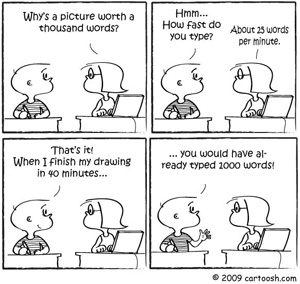
\includegraphics[height=3.5cm]{../images/PictureWords.jpg}
\end{center}
\href{www.abpublish.co.uk/blogphotos/picture_thousand_words.jpg}{\beamergotobutton{Source}}
\end{frame}


\begin{frame}{How to choose an appropriate graphical summary?}
The critical question is: `How can I visually represent this data?' or `What plot will best highlight features of the data?'. This knocks out pie charts and 3D charts!

\vspace{.5cm}
To some extent we use trial and error. We try some standard forms and see what is revealed about the data. One graphical summary can suggest another, and often a combination will highlight different features of the data

\vspace{.5cm}
In practise we use computer packages like R to construct summaries.
However, it is important to understand how to construct graphical summaries ‘by hand’, so that you understand how to interpret computer output and for your final exam. Some computer packages vary slightly in construction. For example, in the calculation of the quartiles or the length of the whiskers in the boxplot.
\end{frame}


\subsection[]{Summary0: Barplot}
\begin{frame}[fragile]{Summary0: Barplot (Categorical data)}

{\bf Q: What was the most common day of road fatality?}

{\tiny 
\begin{knitrout}
\definecolor{shadecolor}{rgb}{0.969, 0.969, 0.969}\color{fgcolor}\begin{kframe}
\begin{alltt}
\hlstd{DayWeek} \hlkwb{<-} \hlstd{data}\hlopt{$}\hlstd{Dayweek}
\hlkwd{table}\hlstd{(DayWeek)}
\end{alltt}
\begin{verbatim}
## DayWeek
##    Friday    Monday  Saturday    Sunday  Thursday   Tuesday Wednesday 
##        68        50        85        56        58        67        58
\end{verbatim}
\begin{alltt}
\hlkwd{plot}\hlstd{(}\hlkwd{table}\hlstd{(DayWeek),}\hlkwc{las}\hlstd{=}\hlnum{2}\hlstd{)}
\end{alltt}
\end{kframe}
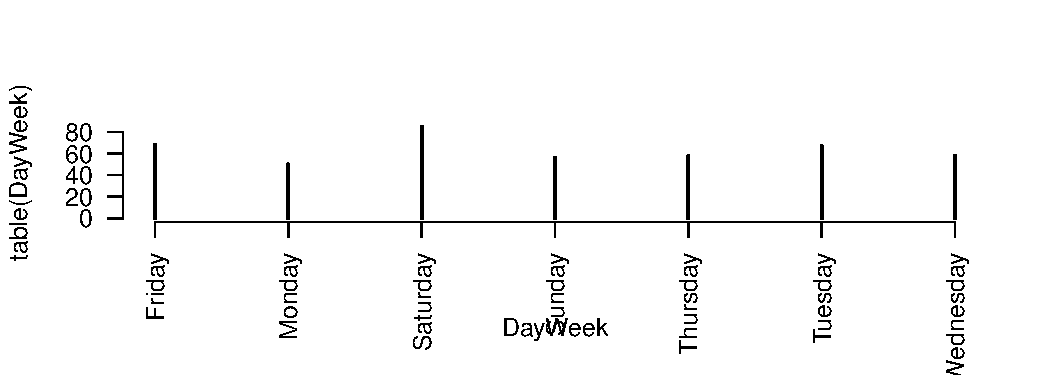
\includegraphics[width=\maxwidth]{figure/unnamed-chunk-5-1} 

\end{knitrout}
}
\end{frame}


\subsection[]{Summary1: Frequency table and ordinate diagram}
\begin{frame}[fragile]{Summary1: Frequency table and ordinate diagram (discrete data)}

{\bf Q: What was the most common speed at which a road fatality occurred?}

\vspace{.5cm}
The frequency table is a very simple way to summarise a set of discrete data and when plotted gives an ordinate diagram. 

\vspace{1cm}
\begin{tabular}{l|llllll|l} \hline
Speed & -9 & 40 & 50 & \ldots & 130 & 888 & Total \\ \hline
Frequency & 28 & 4  & & & &  1 &  442 \\ \hline
\end{tabular}

\vspace{.5cm}
What is strange? Why?
\end{frame}

\begin{frame}[fragile]{}
\begin{knitrout}
\definecolor{shadecolor}{rgb}{0.969, 0.969, 0.969}\color{fgcolor}\begin{kframe}
\begin{alltt}
\hlstd{Speed} \hlkwb{<-} \hlstd{data}\hlopt{$}\hlstd{SpeedLimit}  \hlcom{#Extracts SpeedLimit}
\hlkwd{table}\hlstd{(Speed)}
\end{alltt}
\begin{verbatim}
## Speed
##  -9  40  50  60  70  80  90 100 110 130 888 
##  28   4  53  70  21  53  10 128  71   3   1
\end{verbatim}
\begin{alltt}
\hlkwd{plot}\hlstd{(}\hlkwd{table}\hlstd{(Speed))}
\end{alltt}
\end{kframe}
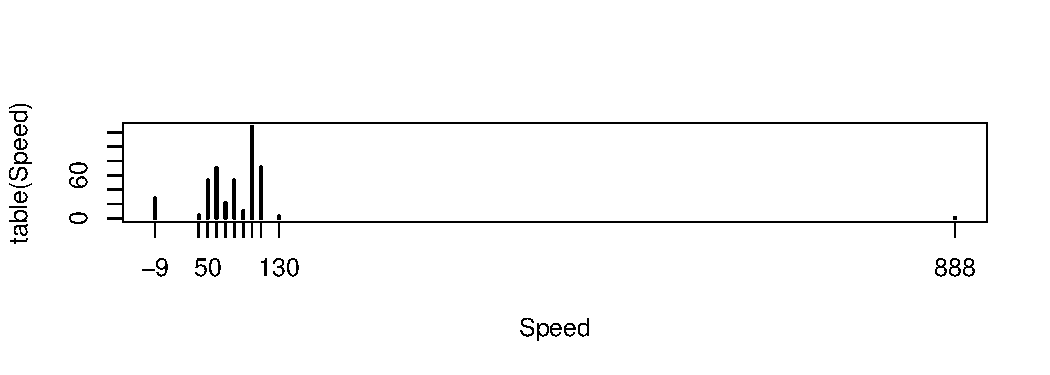
\includegraphics[width=\maxwidth]{figure/unnamed-chunk-6-1} 

\end{knitrout}
\end{frame}

\subsection[]{Summary2: Frequency table and histograms}
\begin{frame}[fragile]{Summary2: Frequency table and histograms (continuous data)}

{\bf Q: What were the most common ages at which a road fatality occurred?}

\vspace{.5cm}
The frequency table can also be used to summarise a set of continuous data, by collecting it into intervals (or ‘bins’). What is lost?

\begin{itemize}
\item 
For equal bin lengths, we can simply sort the data into the bins, and then plot the frequency against each bin. This is called a `regular' histogram. 

\item
For unequal bin lengths, we need to sort the data into the bins, then work out the relative frequency (=frequency/sample size) and the height (=relative frequency/interval length). Plotting the height against each bin is called a 'probability' histogram.
\end{itemize}
\end{frame}

\begin{frame}[fragile]{}

{\bf (i) Using equal bins: Regular Histogram} \\

\begin{center}
\begin{tabular}{| l | l| } \hline
\mbox{Bin} & \mbox{Frequency} \\ \hline
[-10,0) & ? \\ \hline
[0,10) & 11  \\ \hline
[10,20) &  \\ \hline
\ldots &  \\ \hline
[90,100) & 9  \\ \hline
\end{tabular} 
\end{center}

\begin{knitrout}
\definecolor{shadecolor}{rgb}{0.969, 0.969, 0.969}\color{fgcolor}\begin{kframe}
\begin{alltt}
\hlstd{Age} \hlkwb{<-} \hlstd{data}\hlopt{$}\hlstd{Age}
\hlkwd{min}\hlstd{(Age)}
\end{alltt}
\begin{verbatim}
## [1] -9
\end{verbatim}
\begin{alltt}
\hlkwd{max}\hlstd{(Age)}
\end{alltt}
\begin{verbatim}
## [1] 96
\end{verbatim}
\end{kframe}
\end{knitrout}
\end{frame}

\begin{frame}[fragile]{}
\begin{knitrout}
\definecolor{shadecolor}{rgb}{0.969, 0.969, 0.969}\color{fgcolor}\begin{kframe}
\begin{alltt}
\hlstd{Age} \hlkwb{<-} \hlstd{data}\hlopt{$}\hlstd{Age}
\hlkwd{hist}\hlstd{(Age,}\hlkwc{xlab}\hlstd{=}\hlstr{"Age"}\hlstd{,}
     \hlkwc{main}\hlstd{=}\hlstr{"Regular Histogram for Age of Fatality"}\hlstd{)}
\end{alltt}
\end{kframe}
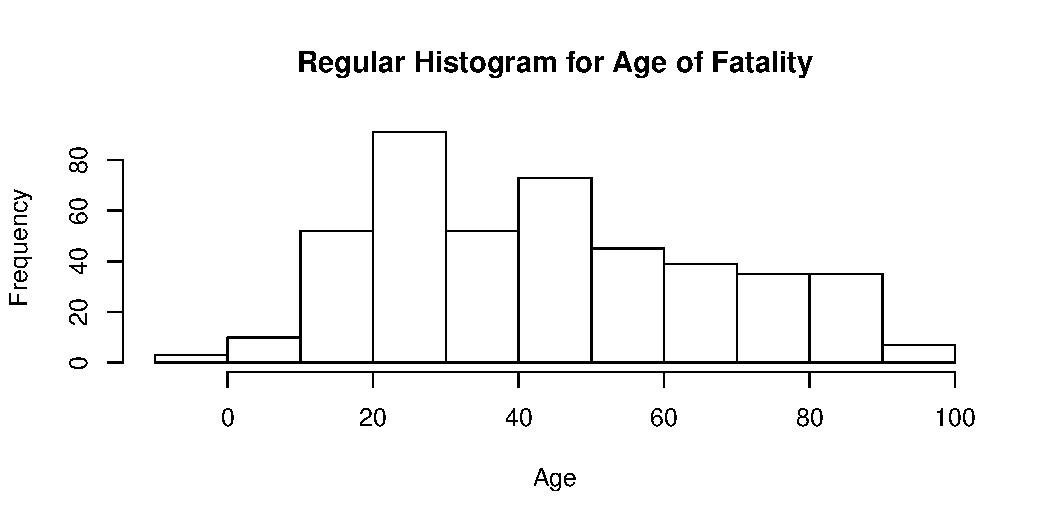
\includegraphics[width=\maxwidth]{figure/unnamed-chunk-8-1} 

\end{knitrout}
\end{frame}

\begin{frame}[fragile]{}

{\bf (ii) Using unequal bins: Probability Histogram} \\

\begin{center}
\begin{tabular}{| l | l| l| l| } \hline
\mbox{Bin} & \mbox{Frequency} & \mbox{Relative Frequency} & \mbox{Height} \\ \hline
[-10,18) & 31  & 31/442 = 0.07 & 0.0025  \\ \hline
[18,25) & 72  & 72/442 = 0.16 & 0.0232 \\ \hline
[25,70) & 259  & 259/442 = 0.59 &  0.0130 \\ \hline
[70,100) & 80  &  80/442 = 0.18 & 0.0060 \\ \hline
Total & 442 & 1 & \\ \hline
\end{tabular} 
\end{center}

where: \\
Relative Frequency = Frequency/442 \\
Height = Relative Frequency/Bin length \\
Eg For bin [-10,18): height = 0.07/28 =3.6. \\
\end{frame}

\begin{frame}[fragile]{}
\begin{knitrout}
\definecolor{shadecolor}{rgb}{0.969, 0.969, 0.969}\color{fgcolor}\begin{kframe}
\begin{alltt}
\hlstd{breaks}\hlkwb{=}\hlkwd{c}\hlstd{(}\hlopt{-}\hlnum{10}\hlstd{,}\hlnum{18}\hlstd{,}\hlnum{25}\hlstd{,}\hlnum{70}\hlstd{,}\hlnum{100}\hlstd{)}
\hlkwd{table}\hlstd{(}\hlkwd{cut}\hlstd{(Age,breaks,}\hlkwc{right}\hlstd{=F))}
\end{alltt}
\begin{verbatim}
## 
## [-10,18)  [18,25)  [25,70) [70,100) 
##       31       72      259       80
\end{verbatim}
\begin{alltt}
\hlkwd{hist}\hlstd{(Age,}\hlkwc{br}\hlstd{=breaks,}\hlkwc{freq}\hlstd{=F,}\hlkwc{right}\hlstd{=F,}
     \hlkwc{xlab}\hlstd{=}\hlstr{"Age"}\hlstd{,}
     \hlkwc{main}\hlstd{=}\hlstr{"Probability Histogram for Age of Fatality"}\hlstd{)}
\end{alltt}
\end{kframe}
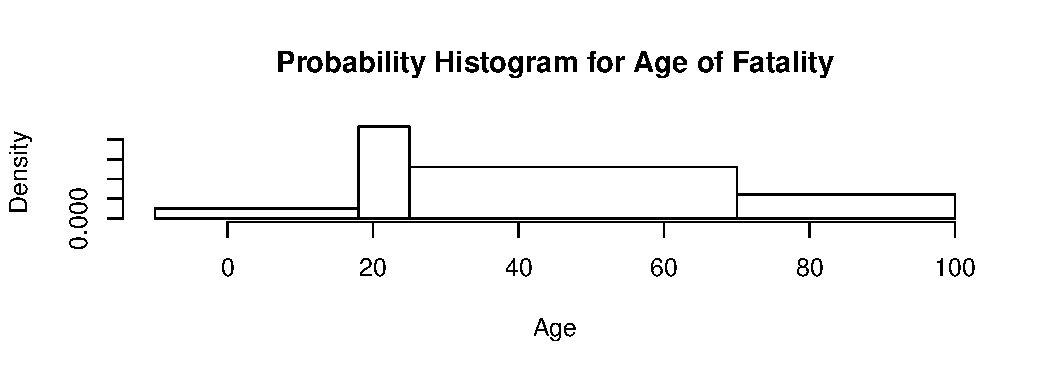
\includegraphics[width=\maxwidth]{figure/unnamed-chunk-9-1} 

\end{knitrout}
\end{frame}

\begin{frame}[fragile]{}
Note how the `regular' histogram is misleading for unequal bin lengths, as it suggests that [25,70) is the most likely bin.

%Gives warning message, hence input pdf following.
%<<fig.height=3,echo=F, results='hide',message=FALSE>>=
%breaks=c(-10,18,25,70,100)
%table(cut(Age,breaks,right=F))   
%hist(Age,br=breaks,freq=T, right=F, main ="Misleading Regular Histogram")  

\vspace{.5cm}
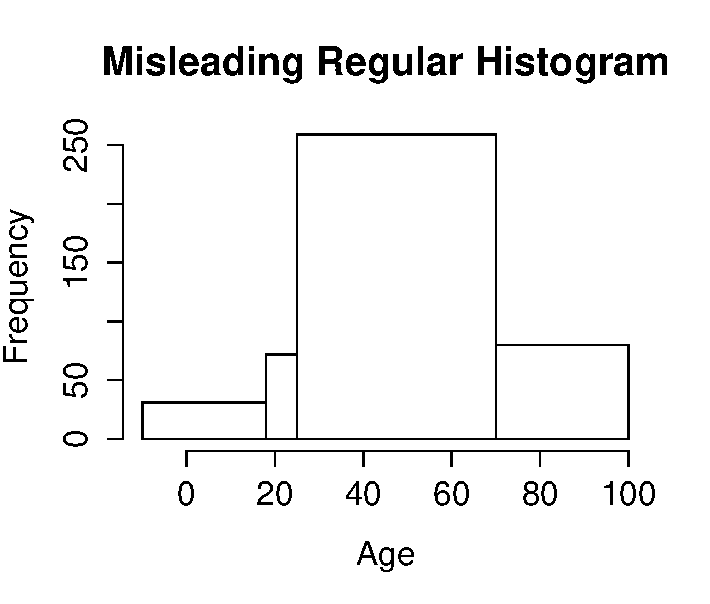
\includegraphics[height=6cm]{../images/AgeMisleadingHist.pdf}
\end{frame}

\subsection[]{Summary3: Stem and leaf plot}
\begin{frame}[fragile]{Summary3: Stem and leaf plot}

{\bf Q: What were the 3 highest ages at which a road fatality occurred?}

\vspace{.5cm}
A stem and leaf plot is basically a histogram turned on its side. It is useful for moderately sized data sets. It provides both a sense of the shape and an ordering of the data, while retaining all the raw numerical data (up to a certain decimal place). 

\vspace{.5cm}
The value to the left of the $\mid$ is called the ‘stem’ and the values on the right are called ‘leaves’.
The leaves should be ordered, although sorting will not affect the shape of the plot.
\end{frame}

\begin{frame}[fragile]{}

{\tiny 
\begin{knitrout}
\definecolor{shadecolor}{rgb}{0.969, 0.969, 0.969}\color{fgcolor}\begin{kframe}
\begin{alltt}
\hlkwd{stem}\hlstd{(Age)}
\end{alltt}
\begin{verbatim}
## 
##   The decimal point is 1 digit(s) to the right of the |
## 
##   -0 | 99
##    0 | 011124557
##    1 | 0034555677777777777788888888888888999999999
##    2 | 00000000000111111222222222223333333333444444444445555555555566666666+12
##    3 | 000000000011111222223333333334445556666666667777778888899
##    4 | 00000111111222222233333333344444444444555555556666666666777777788888
##    5 | 00011111233333344455556777777888888889999
##    6 | 0000000111111122233334445555677788899999999
##    7 | 00011122333444444555556666777788899
##    8 | 000111112222222223333344467788888999
##    9 | 001222336
\end{verbatim}
\end{kframe}
\end{knitrout}
}

Note that R defaults to what it considers to be a sensible layout of the data. Here R chooses a `single' stem plot: with each stem having the leaves 0,1,2,...9. So the reading 2 $\mid$ 3 is age 23. If we consider the data is over-condensed (too stretched out) or under-condensed (too bunched up), we can adjust the format by experimenting with {\tt scale=}.
\end{frame}


\begin{frame}[fragile]{}

{\tiny 
\begin{knitrout}
\definecolor{shadecolor}{rgb}{0.969, 0.969, 0.969}\color{fgcolor}\begin{kframe}
\begin{alltt}
\hlkwd{stem}\hlstd{(Age,}\hlkwc{scale}\hlstd{=}\hlnum{0.25}\hlstd{)}
\end{alltt}
\begin{verbatim}
## 
##   The decimal point is 1 digit(s) to the right of the |
## 
##   -0 | 99
##    0 | 0111245570034555677777777777788888888888888999999999
##    2 | 00000000000111111222222222223333333333444444444445555555555566666666+69
##    4 | 00000111111222222233333333344444444444555555556666666666777777788888+36
##    6 | 00000001111111222333344455556777888999999990001112233344444455555666
##    8 | 000111112222222223333344467788888999001222336
\end{verbatim}
\end{kframe}
\end{knitrout}
}
This is called a double leaf plot, as the stem `0' now has the leaves 0,1,2,3,4 5,6,7,8,9 (representing 00-09) and then a second set of leaves 0,1,2,3,4 5,6,7,8,9 (representing 10-19).  Note you need to read carefully, as 8|0 can represent both 80 or 90.

\vspace{.5cm}
A double stem plot would have one stem `0' with leaves 0,1,2,3,4 (representing 00-04) and then a second stem 'O' with leaves 5,6,7,8,9 (representing 05-09).
\end{frame}

\subsection[]{Summary4: Boxplot}
\begin{frame}[fragile]{Summary4: Boxplot}

\vspace{.5cm}
{\bf Q: Were there any unusual ages at which a road fatality occurred? Is there any difference between the ages of male and female fatalities?}

\vspace{.5cm}
Boxplots are useful for comparing data sets and identifying outliers. 

\begin{knitrout}
\definecolor{shadecolor}{rgb}{0.969, 0.969, 0.969}\color{fgcolor}\begin{kframe}
\begin{alltt}
\hlkwd{boxplot}\hlstd{(Age,}\hlkwc{horizontal}\hlstd{=T)}
\end{alltt}
\end{kframe}
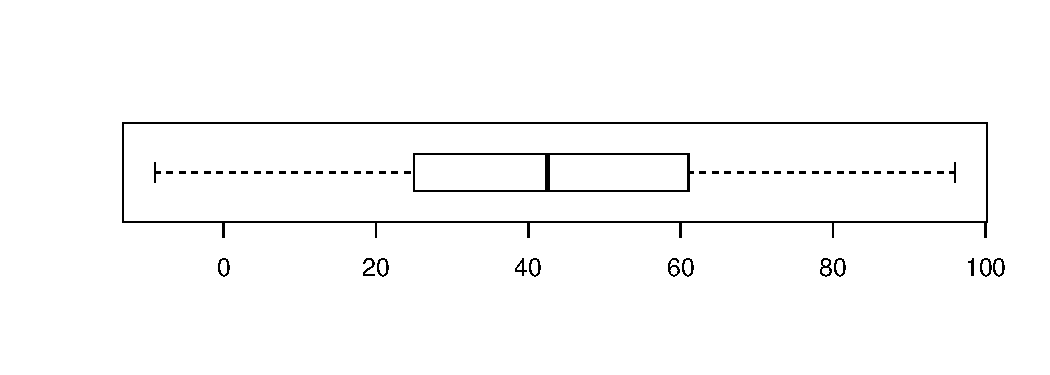
\includegraphics[width=\maxwidth]{figure/unnamed-chunk-12-1} 

\end{knitrout}
 
\end{frame}

\begin{frame}[fragile]{}
\begin{knitrout}
\definecolor{shadecolor}{rgb}{0.969, 0.969, 0.969}\color{fgcolor}\begin{kframe}
\begin{alltt}
\hlstd{AgeM} \hlkwb{<-} \hlstd{data}\hlopt{$}\hlstd{Age[ data}\hlopt{$}\hlstd{Gender} \hlopt{==} \hlstr{"Male"}\hlstd{]}
\hlstd{AgeF} \hlkwb{<-} \hlstd{data}\hlopt{$}\hlstd{Age[ data}\hlopt{$}\hlstd{Gender} \hlopt{==} \hlstr{"Female"}\hlstd{]}
\hlkwd{par}\hlstd{(}\hlkwc{mfrow} \hlstd{=} \hlkwd{c}\hlstd{(}\hlnum{1}\hlstd{,} \hlnum{2}\hlstd{))}  \hlcom{#Puts 2 boxplots in a row}
\hlkwd{boxplot}\hlstd{(AgeM)}
\hlkwd{boxplot}\hlstd{(AgeF)}
\end{alltt}
\end{kframe}
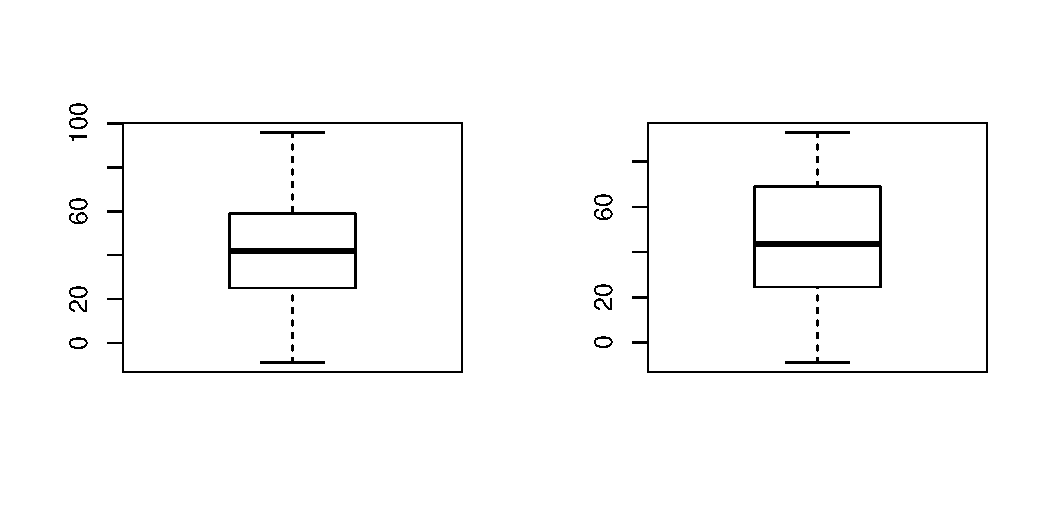
\includegraphics[width=\maxwidth]{figure/unnamed-chunk-13-1} 

\end{knitrout}
\end{frame}

\begin{frame}[fragile]{}

A neat trick for producing the same boxplots:
\begin{knitrout}
\definecolor{shadecolor}{rgb}{0.969, 0.969, 0.969}\color{fgcolor}\begin{kframe}
\begin{alltt}
\hlkwd{boxplot}\hlstd{(Age}\hlopt{~}\hlstd{data}\hlopt{$}\hlstd{Gender,} \hlkwc{ylab}\hlstd{=}\hlstr{"Age"}\hlstd{)}
\end{alltt}
\end{kframe}
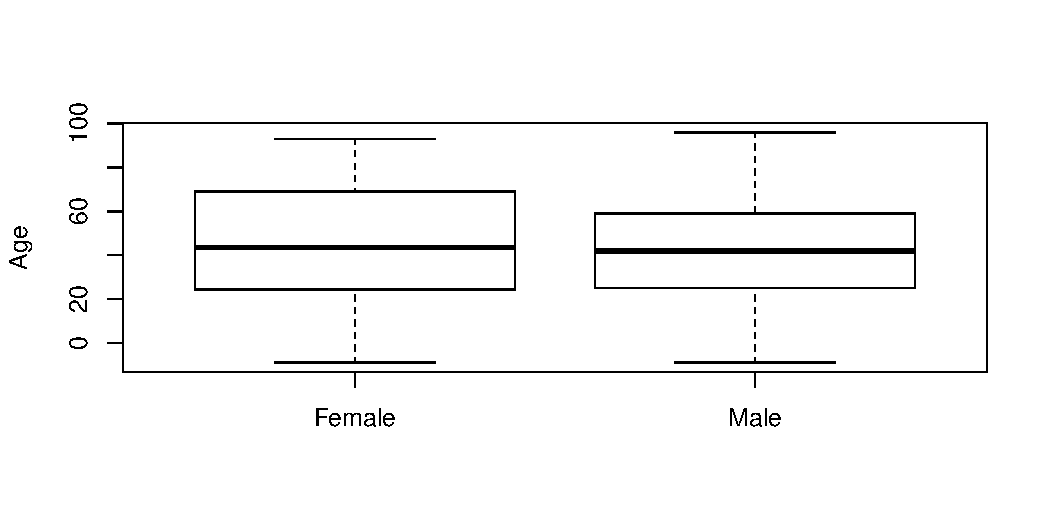
\includegraphics[width=\maxwidth]{figure/unnamed-chunk-14-1} 

\end{knitrout}
\end{frame}


\begin{frame}[fragile]{}

The boxplots show that the ages of road fatalities for men and women is similar.
However, what do we learn from this simple commmand?

\begin{knitrout}
\definecolor{shadecolor}{rgb}{0.969, 0.969, 0.969}\color{fgcolor}\begin{kframe}
\begin{alltt}
\hlkwd{length}\hlstd{(AgeM)}
\end{alltt}
\begin{verbatim}
## [1] 326
\end{verbatim}
\begin{alltt}
\hlkwd{length}\hlstd{(AgeF)}
\end{alltt}
\begin{verbatim}
## [1] 116
\end{verbatim}
\end{kframe}
\end{knitrout}
\end{frame}

\begin{frame}[fragile]{}

{\bf Q: What were there any unusual speeds at which fatalities occurred?}

\begin{knitrout}
\definecolor{shadecolor}{rgb}{0.969, 0.969, 0.969}\color{fgcolor}\begin{kframe}
\begin{alltt}
\hlkwd{boxplot}\hlstd{(data}\hlopt{$}\hlstd{SpeedLimit,} \hlkwc{horizontal} \hlstd{= T)}
\end{alltt}
\end{kframe}
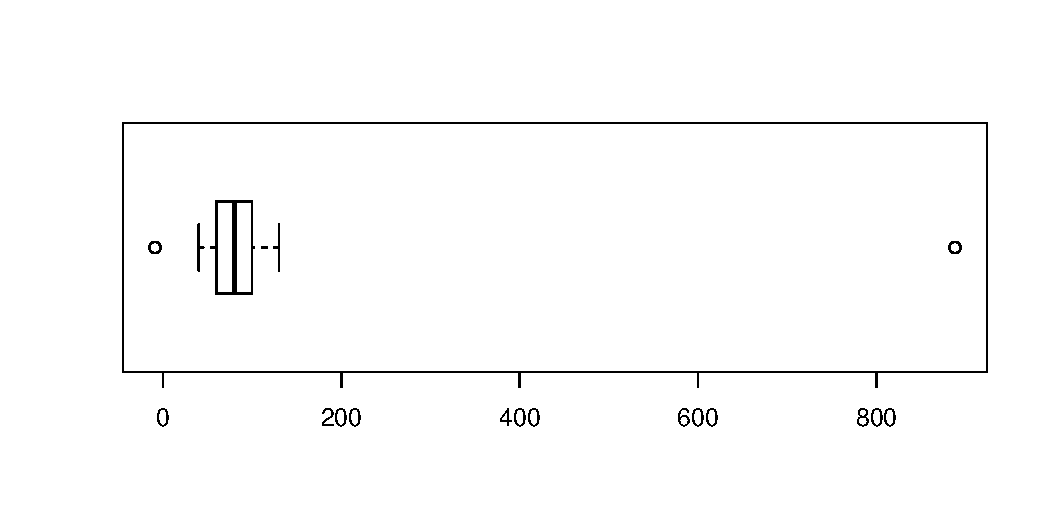
\includegraphics[width=\maxwidth]{figure/unnamed-chunk-16-1} 

\end{knitrout}
\end{frame}

\begin{frame}[fragile]{}
\vspace{.5cm}
A box plot is a visual representation of the 5 number summary
(min, $Q_1$= 1st quartile, $Q_2$= median, $Q_3$= 3rd quartile, max), where:

\begin{itemize}
\item Min = smallest data point(s) \\
\item Max = largest data point(s) \\
\item $Q_2$ = middle data point (find the average of the 2 middle points for even sized dataset.) \\
\item $Q_{1}$ and $Q_{3}$ are the `medians' of the half data sets: we divide the data into 2 sets at the median (including the median for an odd sized data set), and then find the median of each half set of data.
\end{itemize}

See more fuller definitions:  \hyperlink{Quartiles}{\beamergotobutton{Quartiles}} 

\end{frame}


\begin{frame}[fragile]{}

There are different conventions for boxplots. We will use the convention that the whiskers extend to the minimum and maximum observations within the thresholds [LT,UT], where 
\begin{itemize}
\item Lower Threshold $LT=Q_1-1.5IQR$;
\item Upper Threshold $UT=Q_3+ 1.5IQR$;
\item Interquartile range is $IQR=Q_3-Q_1$.
\end{itemize}

\vspace{.5cm}
An outlier is any observation lying outside of [LT,UT].
\end{frame}


\begin{frame}[fragile]{}
\vspace{1cm}
\begin{tikzpicture}[thick, framed]
    \filldraw[fill=green!20] (2,0) rectangle (5,1);% draw the box
    \draw (3,0) -- (3,1) node[above]{$\textsc{Q2}$};% draw the median
    \draw (5,0.5) -- (7,0.5);% draw right whisker
    \draw (2,0.5) -- (1,0.5);% draw left whisker
    \draw (7,0.39) -- (7,0.61);% draw vertical tab
    \draw (1,0.39) -- (1,0.61);% draw vertical tab
    \node[below] at (2,0) {$\textsc{Q1}$};% label the hinge
    \node[below] at (5,0) {$\textsc{Q3}$};% label the hinge
    \filldraw[ball color=red!80,shading=ball] (4,0.5) circle
        (0.06cm) node[above]{$\bar{x}$};% the mean
    \draw[<->] (2.3, -0.3) -- (4.7, -0.3)
        node[pos=0.5,below]{$\textsc{IQR}$}; % mark the IQR fences
    \draw[<->] (2, -0.8) -- (0,-0.8)
        node[pos=0.5,below]{$\textsc{1.5*IQR}$}; % left inner fence
  %  \draw[<->] (2,-1.4) -- (-2, -1.4)
  %      node[pos=0.5,below]{$\textsc{3*IQR}$};% left outer fence
    \draw[<->] (5, -0.8) -- (8,-0.8)
        node[midway,below]{$\textsc{1.5*IQR}$}; % right inner fence
  %  \draw[<->] (5,-1.4) -- (10, -1.4)
   %     node[pos=0.5,below]{$\textsc{3*IQR}$};% right outer fence
    %
  %  \node[below] at (7.5,0.7) {$o$}; % mild outlier on the right
    \node[below] at (0,0.7) {$o$}; % extreme outlier on the left
    % Title
    \draw (3,2) node[above,xshift=0.7cm]{$ \textsc{Box
        Plot}$};%
    % Axis
  %  \draw (-3,-2) -- (8,-2);
    % Note that the snaked line is drawn to 11.1 to force
    % TikZ to draw the final tick.
  %  \draw[snake=ticks,segment length=1cm] (-3,-2) -- (8.1,-2);
\end{tikzpicture}

\vspace{.5cm}
Note: Here we have indicated the mean $\bar{x}$ in red for comparision with the median $Q_{2}$, but normally that is not shown on the boxplot.
\end{frame}

\begin{frame}[fragile]{Steps for Constructing a Boxplot by Hand}
\begin{enumerate}
\item Calculate the quartiles $Q_1$, $Q_2$ and $Q_3$ and the interquartile range $IQR$. 
\item Draw a box from $Q_1$ to $Q_3$, with a line within the box for the median= $Q_2$.
\item Calculate the upper and lower thresholds.
\item Draw a whisker from the box to the nearest points within the thresholds.
\item Any points outside the thresholds are outliers, designated by circles.
\end{enumerate}
\end{frame}

\subsection[]{Describing the Shape of Data}
\begin{frame}[fragile]{Describing the Shape of Data}

When we look at graphical summaries, we want to describe the form of the data and any ‘idiosyncrasies’.

\vspace{.5cm}
3 key questions:

1. Is it symmetric or skewed?
\begin{knitrout}
\definecolor{shadecolor}{rgb}{0.969, 0.969, 0.969}\color{fgcolor}
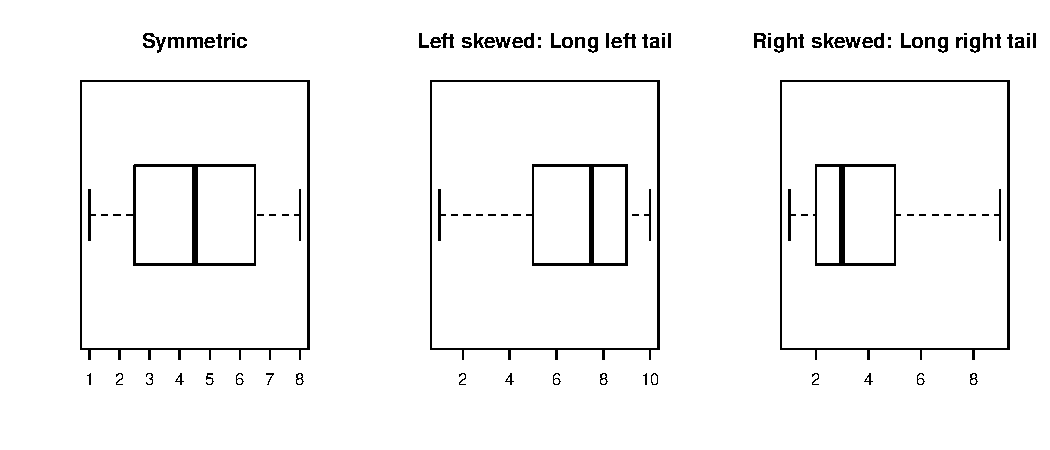
\includegraphics[width=\maxwidth]{figure/unnamed-chunk-17-1} 

\end{knitrout}
\end{frame}

\begin{frame}[fragile]{}

2. Is it unimodal, bimodal, trimodal, multimodal or other?
\begin{knitrout}
\definecolor{shadecolor}{rgb}{0.969, 0.969, 0.969}\color{fgcolor}
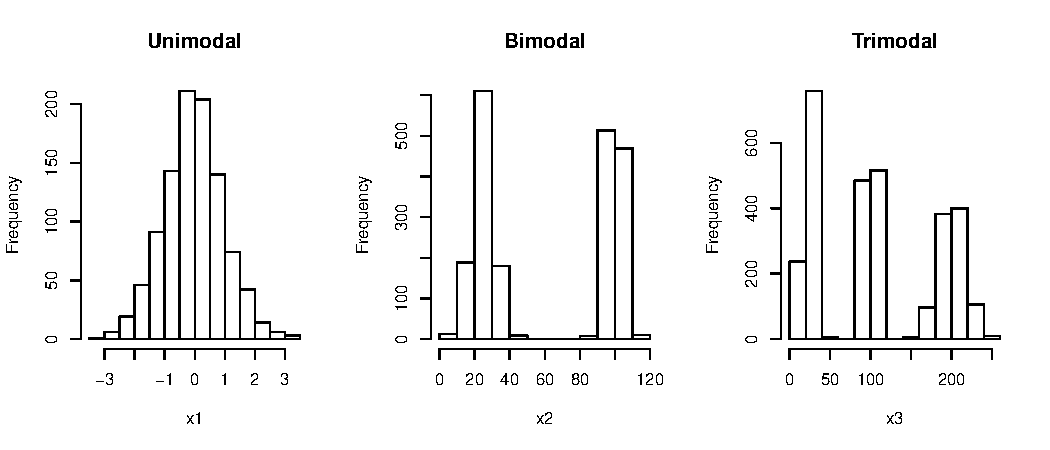
\includegraphics[width=\maxwidth]{figure/unnamed-chunk-18-1} 

\end{knitrout}

Note: Bimodality can be an indication of interesting behaviour to explore. However, it can also arise from 2 populations mistakingly put together. 
\end{frame}

\begin{frame}[fragile]{}

3. Are there any unusual features?  (eg outliers or gaps)
\begin{knitrout}
\definecolor{shadecolor}{rgb}{0.969, 0.969, 0.969}\color{fgcolor}
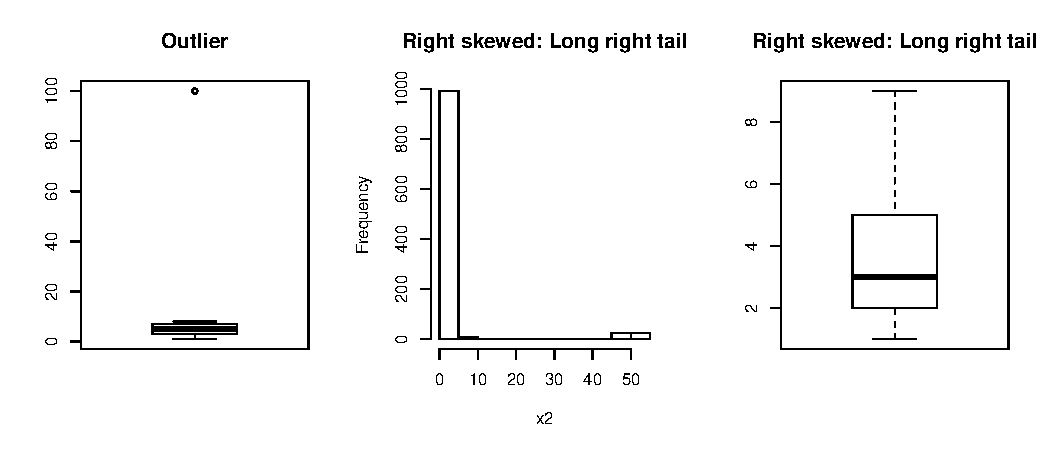
\includegraphics[width=\maxwidth]{figure/unnamed-chunk-19-1} 

\end{knitrout}


Note: An outlier needs to be investigated carefully, as it can be an indication of an interesting data point or possibly a mistake in the recording of data.
\end{frame}


\subsection[]{Dirty Data}
\begin{frame}[fragile]{Dirty Data}

Notice that throughout Topic1 we have deliberately showcased raw data with the missing values coded as '-9'. This is called 'dirty data' and is how real data exists. 

\vspace{.5cm}
Dealing with 'dirty data' is outside the scope of MATH1005, as it can require some sophistication. Ideally, we would replace all the missing values by a blank. However, one possible strategy is to account for the missing values in your histogram: create the bins (-10,0), [0,18] ..., so there is effectively 1 nonsense bin (although it still affects the calculation of frequencies of the other bins.)
\end{frame}






\end{document}
